The goal of this chapter is to discuss the performance of Bacco, using a variery of parameters, methods and laboratory
tests. The results will also be compared to the ones obtained by applying the same procedures to devices using the
LoRaWAN protocol.

\section{Time On Air}
\Gls{ToA} is a crucial metric to take into consideration when measuring the performance of a network protocol. It is
defined as time that a device takes to transmit a packet on the channel. At the same conditions, a shorter \gls{ToA}
results in improved energy efficiency and smaller probability of interference with packets transmitted from other
devices.\\
\Gls{ToA} is directly proportional to the packet lenght (longer packets will require more symbols to encode them), so in
order to reduce \gls{ToA} without changing the modulation, it is necessary to reduce the number of bytes to
represent the information contained in each packet.

\subsection{Regulations}
\label{subsec: regulations}
In order to maintain a fair distribution of the transmission activity, local, national and international governments
define limits on the usage of the radio channel. The limits vary by the frequency that the devices operate at.
The two parameters that are often used as an upper bound not to be crossed are \gls{ERP}\footnote{\gls{ERP} is the
measure of the power effectively radiated by an antenna system in a specific direction, accounting for both transmitter
output and antenna characteristic. It is commonly expressed in watts or decibel and it is used for determining the coverage area
and range of a radio.} and duty cycle. The duty cycle is the fraction or percentage of time in which the channel
is busy, it is gived by $d = \frac{\tau}{T}$, where $d$ is the duty cycle, $\tau$ is the \gls{ToA} and $T$ is the
transmission period.\\
Taking the current Italian regulation at the time of writing as an example, we can observe that the spectrum is split into
frequency bands, and each of them has three parameters associated to it: the maximum \gls{ERP}, the minimum channel
distance in terms of frequency and the maximum duty cycle. The official document that discusses this matter in detail can
be found in \cite{gazzetta_potenza_868}. The bands that LoRa devices use in Europe are $\[868.0,868.6\]$ MHz and
$\[868.7,869.2\]$ MHz, they both feature a maximum \gls{ERP} of 25 mW or 14 dBm and do not have any restriction on
channel usage, however the first band has a maximum duty cycle of 1\%, while for the other limit is 0.1\%.\\
An important fact to point out is that the limits apply to a physical person or organization and not to a
single device, so we have to consider the total transmission activity of the network when we calculate the duty cycle.


\subsection{Maximum Number Of Devices In A Network}
Based on the imposed regulations, 

\subsubsection{Bacco}

\subsubsection{LoRaWAN}


\section{Laboratory Tests}

\subsection{Single Packet Energy}

\begin{figure}[ht]
    \centering
    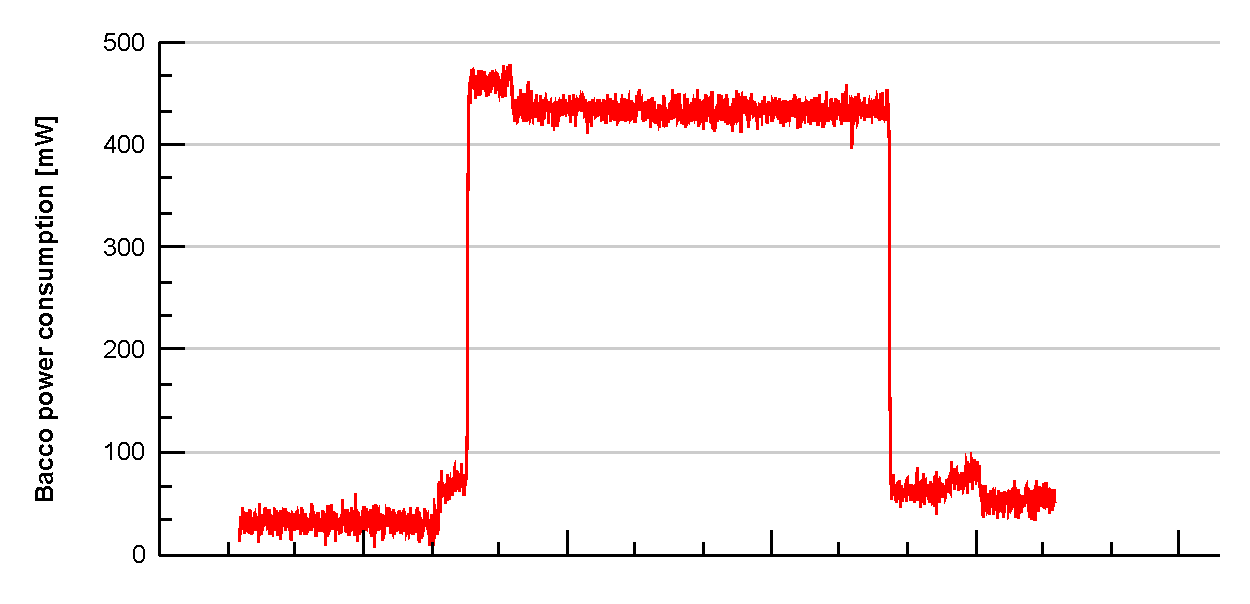
\includegraphics[width=1.0\textwidth]{images/bacco_SF7_14dbm_125khz_power.pdf}\\
    \vspace{-0.7cm}
    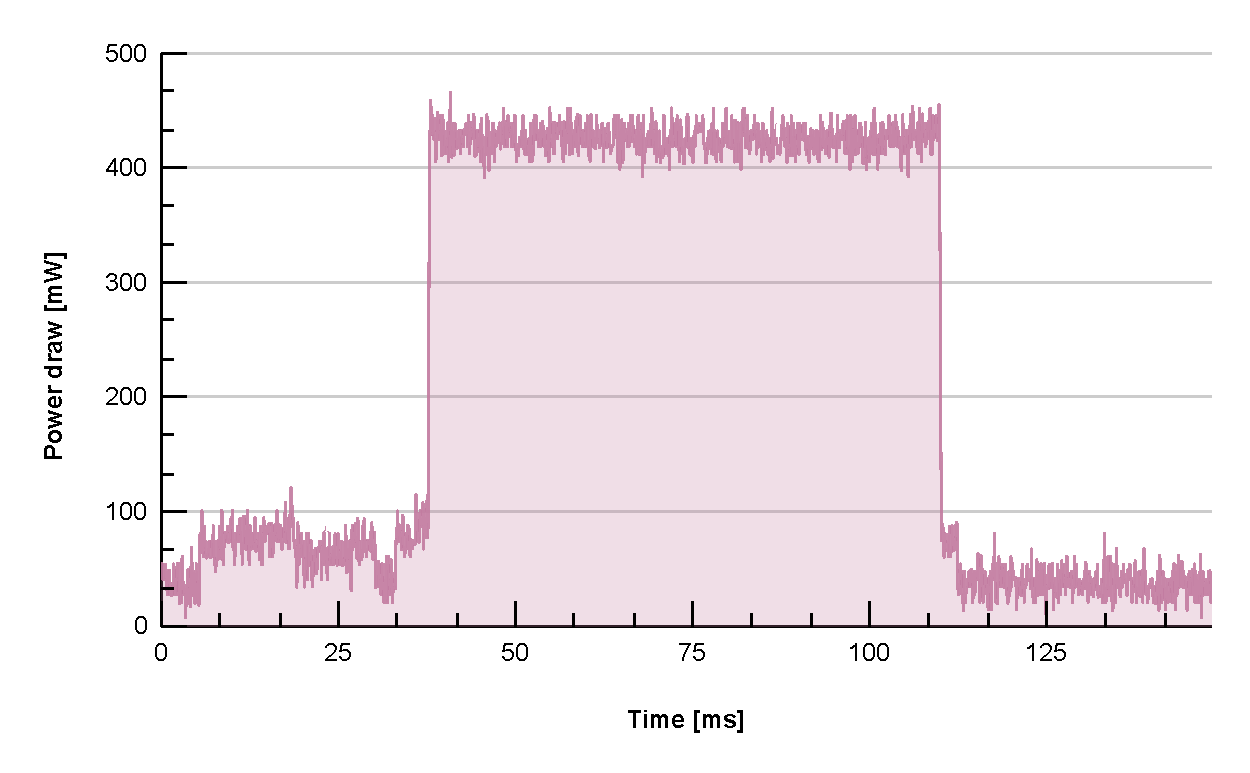
\includegraphics[width=1.0\textwidth]{images/lorawan_SF7_14dbm_125khz_power.pdf}
    \caption{Power draw of Bacco (in red) and LoRaWAN (in blue) during the transmission of a packet with a payload of 15
    bytes, using SF7, 14dBm, 125kHz bandwidth}
    \label{bacco SF7}
\end{figure}

Bacco:\\
delta time is 51.6ms and total energy is 21.3mJ
\\\\
LoRaWAN:\\
delta time is 71.8ms and total energy is 30.8mJ

\subsection{Packet Error Rate}
Crunch some fking data from FTP server

4 lost packets for every 1008 packets (0.4\% biatcz)
%TODO: similar test with fking LoRa fking WAN
